\documentclass[aspectratio=169]{beamer}

\usetheme[
	%titleformat=smallcaps,
	background=dark,
	progressbar=frametitle,
	numbering=none,
]{metropolis}
\usecolortheme{owl}

\usepackage{appendixnumberbeamer}

\usepackage{booktabs}
\usepackage[scale=2]{ccicons}

\usepackage{pgfplots}
\usepgfplotslibrary{dateplot}
\usepackage[]{graphicx}
\usepackage[]{url}
\usepackage[utf8]{inputenc}
\usepackage[]{hyperref}

\usepackage{xspace}
\newcommand{\themename}{\textbf{\textsc{metropolis}}\xspace}

% When using Metropolis
%\setbeamercolor{frametitle}{%
%	fg=black!2,
%	bg=mDarkTeal
%}

%-----8<------------8<------------8<------------8<------------8<------------8<------------

\title{A look into the Mobile Messaging Black Box}
\subtitle{\scriptsize{33rd Chaos Commmunication Congress \#33c3}}
\date{\today}
\author{
	\parbox[t]{1.2in}{Roland Schilling}{\scriptsize{\texttt{@NerdingByDoing}}}\\
	\parbox[t]{1.2in}{Frieder Steinmetz}{\scriptsize{\texttt{@twillnix}}}
}

\institute{Hamburg University of Technology\\
Security in Distributed Applications}
% \titlegraphic{\hfill\includegraphics[height=1.5cm]{logo.pdf}}


%-----8<------------8<------------8<------------8<------------8<------------8<------------

% stuff for arbitrary image placement
% http://tex.stackexchange.com/questions/16357/how-can-i-position-an-image-in-an-arbitrary-position-in-beamer
\tikzset{
  corner node/.style={
    anchor=south east,xshift=-.5cm,yshift=.5cm,
  },
}
\def\tikzoverlay{%
   \tikz[overlay,remember picture]\node[corner node]
}%

%-----8<------------8<------------8<------------8<------------8<------------8<------------

\begin{document}

\maketitle

\section{Introduction}

\begin{frame}
	\frametitle{Messaging - An Analogy}
	\begin{itemize}
		\item You're at a party
		\item Friend approaches you and needs to tell you something \alert{in private}
		\item What do you expect when you say \alert{private}?
		\item You enter a separate room, you trust the location
		\item What does a separate room offer you?
			\begin{itemize}
				\item Confidentiality
				\item Authenticity
				\item Integrity
				\item Forward Secrecy
				\item Future Secrecy
				\item Plausible Deniability
			\end{itemize}
	\end{itemize}
\end{frame}

\begin{frame}
	\frametitle{A Private Room}
	You are now alone in a closed room with your Friend
	\begin{itemize}
		\item Both of you have absolute Confidentiality that you are alone
		\item Nobody can overhear your talk
		\item Your exchange is completely private
	\end{itemize}
	We call this \alert{confidentiality}

	\tikzoverlay at (current page.south east){
		
\includegraphics[width=6cm]{img/conversation.pdf}
	};

\end{frame}


\begin{frame}
	\frametitle{In Sight of Each Other}
	The room you're in is small enough that you can always see each other
	\begin{itemize}
		\item You know that the words you speak are received just as you spoke them
		\item There is no way either of you hears something else that the other says
	\end{itemize}
	We call this \alert{integrity}
\end{frame}

\begin{frame}
	\frametitle{You Know Each Other}
	Since you're long-time friends, you're absolutely sure, whom you're talking to
	\begin{itemize}
		\item Nobody can impersonate your friend or you, without the other noticing
		\item You're talking directly, without a phone or webcam in between
	\end{itemize}
	We call this \alert{authenticity}
\end{frame}

\begin{frame}
	\frametitle{It's a One-Time Talk}
	\only<1>{%
	Suppose somebody was present in the room with you	
	\begin{itemize}
		\item They could overhear your conversation
		\item They would only learn the contents of this particular conversation
		\item They would not learn anything about past conversations you had
	\end{itemize}
	We call this \alert{forward secrecy}
	\begin{itemize}
		\item[$\rightarrow$] They would also not learn anything about future conversations you might have
	\end{itemize}
	We call this \alert{future secrecy}}
	\only<2>{%
		Perfect Forward- and Future Secrecy\\
		\begin{center}
			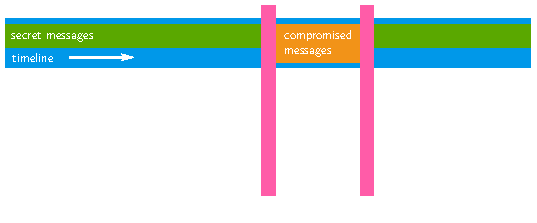
\includegraphics[width=\textwidth]{img/pfs.pdf}
		\end{center}
	}
\end{frame}

\begin{frame}
	\frametitle{It's a One-Time Talk Between Only You Two}
	There are no witnesses in the room
	\begin{itemize}
		\item Either of you can later deny to other having made any statement
		\item Neither of you can prove to other that any of you have made a particular statement
	\end{itemize}
	We call this \alert{deniability}
\end{frame}

\section{Enter Messaging Services}

\begin{frame}
	\frametitle{Messaging}
	\centering
	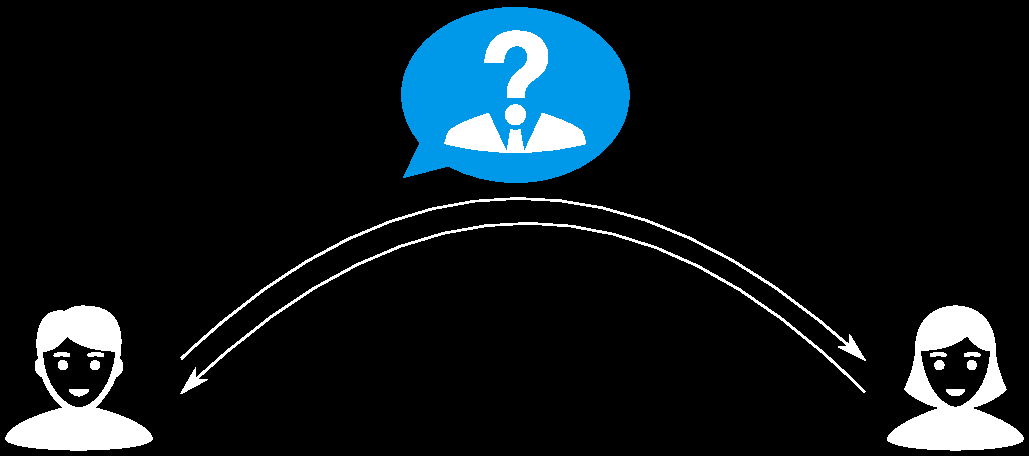
\includegraphics[width=.75\textwidth]{img/messaging.pdf}	
\end{frame}

\begin{frame}
	\frametitle{Messaging}
	Parties involved
	\begin{itemize}
		\item Depending on the scenario, at least one additional party is involved, the messaging provider
		\item push message provider might also be involved
		\item In federated scenarios, multiple relaying parties may be involved
		\item[$\Rightarrow$] Messaging solutions should be designed so as to minimized the data these parties may obtain
	\end{itemize}
	Problems:
	\begin{itemize}
		\item How to find your peers? (address book leakage)
		\item How to relay messages to the recipient? (participation leakage)
		\item Relay always knows the exact time a message was sent
		\item Relay always knows the size of transmitted messages (padding helps)
	\end{itemize}
\end{frame}

\begin{frame}
	\frametitle{Traditional Messaging}
	What if this conversation had taken place via SMS?\\[1em]
	Your providers
	\begin{itemize}
		\item would know the contents of your exchange: \alert{no confidentiality}
		\item could change the contents of your exchange: \alert{no integrity}
		\item could reroute your messages and impersonate either of you: \alert{no authentication}
		\item would know all messages you ever exchanged: \alert{no forward Secrecy}
		\item would know all messages exchanged in the future: \alert{no future secrecy}
		\item could store all messages and use them as proof of the exchange: \alert{no deniability}
	\end{itemize}
	Messaging translates badly to our offline communication expectation
\end{frame}

\section{Case Study - Signal}

\begin{frame}
	\frametitle{Signal - Notes}
	\begin{itemize}
		\item Server-side cached short-term keys (\alert{prekeys}) fetched by sender
		\item Pairwise long-lived symmetric secret key between participants
		\item Multiple messages without answer $\rightarrow$ perform KDF on \alert{chaining key}
		\item ECDH: Curve25519, AES-CTR (no padding), AES-CBC (PKCS7 padding)
		\item HMAC-SHA256 for integrity
		\item Future secrecy only if private keys are not leaked (duh!). Since private keys go into new shared keys during ratcheting, the attacker lacks material to compromise next key after obtaining current one.
		\item Since shared keys are only deleted after messages are received, there is a window in which keys could be compromised before reception. 
		\item Deniability is always a theoretical claim as long as a transmission server has the ability to log messages, their senders and recipients.

	\end{itemize}
\end{frame}

\section{Reverse-Engineering Threema}

\begin{frame}
	\frametitle{Enter Threema}
	Threema
	\begin{itemize}
		\item Gained popularity in Germany after Facebook purchased WhatsApp
		\item All promise -- no proof; first openly contemplating to OSS the code, later backing away from that statement
		\item Interest in its inner workings
	\end{itemize}

	Quick Shoutouts
	\begin{itemize}
		\item Jan Ahrens for releasing his findings about the handshake before we did
		\item OpenMittsu for releasing the first working OSS client
	\end{itemize}
	
\end{frame}

\begin{frame}
	\frametitle{Reverse-Engineering -- What to look for?}
\begin{itemize}
	\item Test for common pitfalls in implementation
		\begin{itemize}
			\item Handling of TLS
			\item Handling of keys and nonces
			\item NaCl implementation errors
			\item Uncommon data leaks
			\item Bugs
			\item \ldots?
		\end{itemize}
	\item Find out how protocol is designed
		\begin{enumerate}
			\item Understand handshakes
			\item Understand protocol
			\item decipher messages
		\end{enumerate}
\end{itemize}
\alert{Positive side-note}: Threema had released a security white paper early on
\end{frame}

\begin{frame}
	\frametitle{Threema - Notes and Open Questions}
	Notes:
	\begin{itemize}
		\item PFS only on transport layer (attacker sniffing packets from the outside will not learn contents after private key acquisition)
	\end{itemize}
	Q:
	\begin{itemize}
		\item How often is the handshake performed?
	\end{itemize}
\end{frame}

\begin{frame}
	\frametitle{Threema Packet Format}

	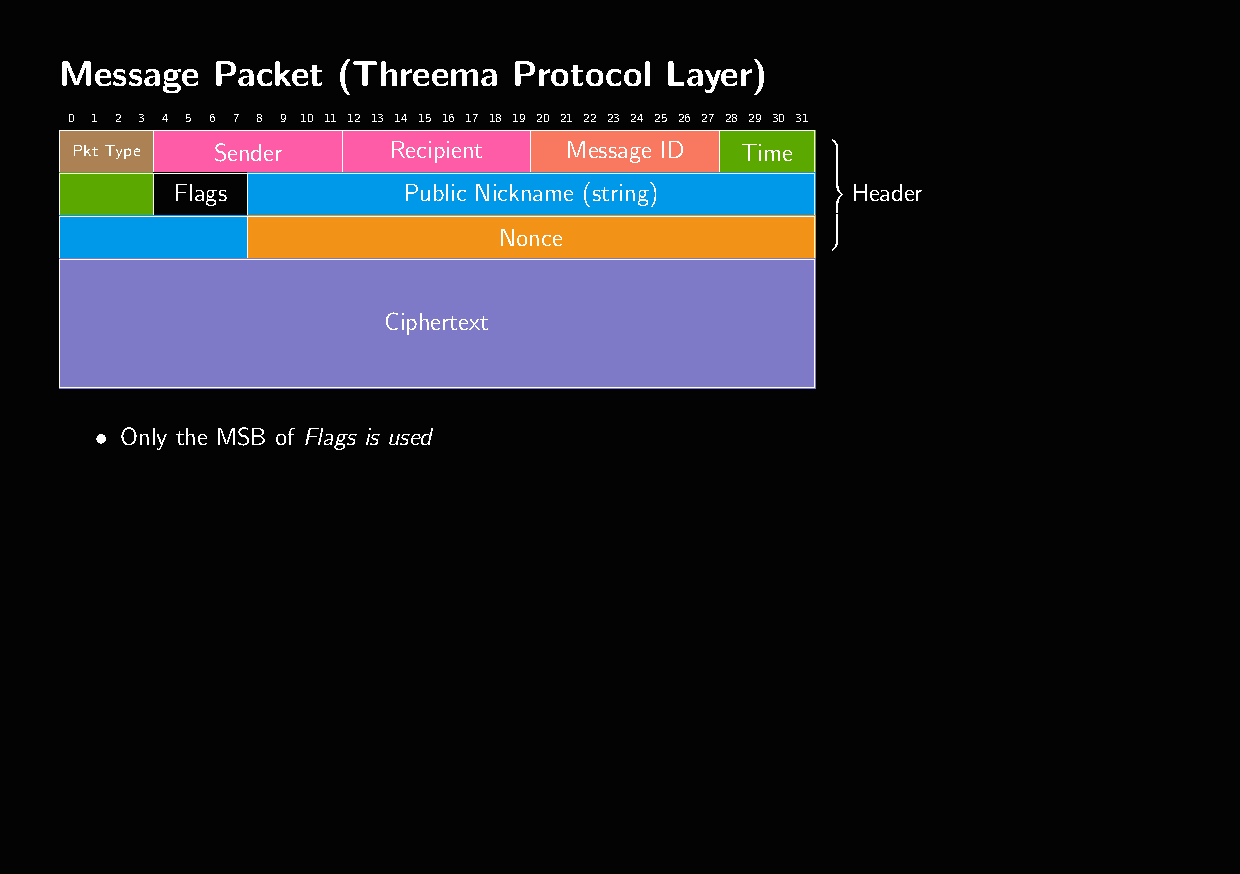
\includegraphics[page=1,clip,trim={.99cm 8cm 3.2cm 1.8cm},width=\textwidth]{out/messages.pdf}

\end{frame}

\begin{frame}
	\frametitle{Threema: Special Messages}
	\begin{itemize}
		\item Polls
		\item Images with Caption
			\begin{itemize}
				\item Case of caption leak found
			\end{itemize}
		\item Audio Messages
			\begin{itemize}
				\item Leak Android version
				\item Possible StageFright vector
			\end{itemize}
	\end{itemize}
\end{frame}

\begin{frame}
	\frametitle{Threema Image Messages}
	\includegraphics[page=4,clip,trim={.99cm 7.5cm 3.2cm 1.8cm},width=\textwidth]{out/messages.pdf}
\end{frame}

\begin{frame}
	\frametitle{Threema Audio Messages}
	\includegraphics[page=5,clip,trim={.99cm 7.5cm 3.2cm 1.8cm},width=\textwidth]{out/messages.pdf}
\end{frame}

\begin{frame}
	\frametitle{Group Messages}
	\includegraphics[page=6,clip,trim={.99cm 7.5cm 3.2cm 1.8cm},width=\textwidth]{out/messages.pdf}
\end{frame}

\begin{frame}
	\frametitle{Done!}
	\Huge{Thank You!}
	%\alert{\rule{\textwidth}{1pt}}\\[2em]
	\\[2em]
	\scriptsize
	\begin{tabular}{@{}lll}
		Roland Schilling & \url{@NerdingByDoing} & \url{schilling@tuhh.de} \\
		Frieder Steinmetz & \url{@twillnix} & \url{frieder.steinmetz@tuhh.de} \\
	\end{tabular}\\[1em]
	\alert{\rule{.75\textwidth}{1pt}}\\[1em]
	\begin{tabular}{@{}ll}
		Beamer Theme: & \alert{\href{https://github.com/matze/mtheme}{Metropolis}} by Matthias volgelsang\\
		Color Theme: & \alert{\href{https://github.com/rchurchley/beamercolortheme-owl}{Owl}} by Ross Chirchley \\
		Icons: & \alert{\href{https://thenounproject.com/mockturtle/collection/big/}{The BIG collection}} by Sergey Demushkin\\
	\end{tabular}\\[3em]
	Thanks to \textbf{Jan Ahrens} and \textbf{Philipp Berger} -- their work has made ours somewhat easier\\
	Thanks to \textbf{Maximilian Köstler} for his initial work on Threema

\end{frame}

\end{document}

% vim: spelllang=en spell
